\section{Channel System}
\label{sec:channelSystem}

With each member being a set of roles, it remains to model a description of how each member communicates with another, exchanging information during the mission. Recalling our motivation example, some requirements are still missing, and need to be addressed. First, during the entire mission, members are communicating with some other entity all the time. This means that parallelism is important to maintain each entity executing its roles, i.e, functionalities, at the same time. For instance, drones that only execute tasks in some particular C2 approach can communicate with the drone that detains the task allocator role, while executing the next task. Most importantly, the drone responsible for allocating tasks can use some protocol to assess the status of the members, e.g, checking if the drone dropped or is fully functional. Likewise, the C2 approach selector and task allocator roles can exchange messages that may cause a new maneuver, caused by context changes.

A channel system is composed of a group of data-dependent processes communicating with each via \textit{communication actions}~\cite{modelcheckingBaier}. With a program graph representing each process, transitions can be classified between conditional transitions, functioning as explained in Section \ref{subsec:PG}, or communication actions. This last type of transition works transmitting values through channels or receiving values from channels and assigning them to variables~\cite{modelcheckingBaier}. Additionally, channels can have a finite or infinite capacity of messages in a single channel, as well as a specified type of messages that can be stored in it. Finally, channel systems provide a notion of synchronization, whereas channels with a capacity different from zero function in a \textit{asynchronous} way and null capacity channels represent \textit{synchronous} communication~\cite{modelcheckingBaier}.

In our motivating example, each member, comprising a set of role's program graphs, is switching between actions related to its function or actions related to communication purposes. To decide which action to take, members update variables to properly evaluate conditions. Thus, when a condition related to some context change becomes true, the member can transmit this feedback to the member that possesses the task allocator role using, for example, the channel \textit{ch1}. If the task allocator decides that the current C2 Approach is not capable of maintaining quality during execution, it can send a maneuver request to C2 approach selector drone, using, for example, channel \textit{ch3}. Figure \ref{fig:CS} illustrates this scenario.

\begin{figure}[!ht]
    \centering
    \scalebox{.75}{

\tikzset{every picture/.style={line width=0.75pt}} %set default line width to 0.75pt        

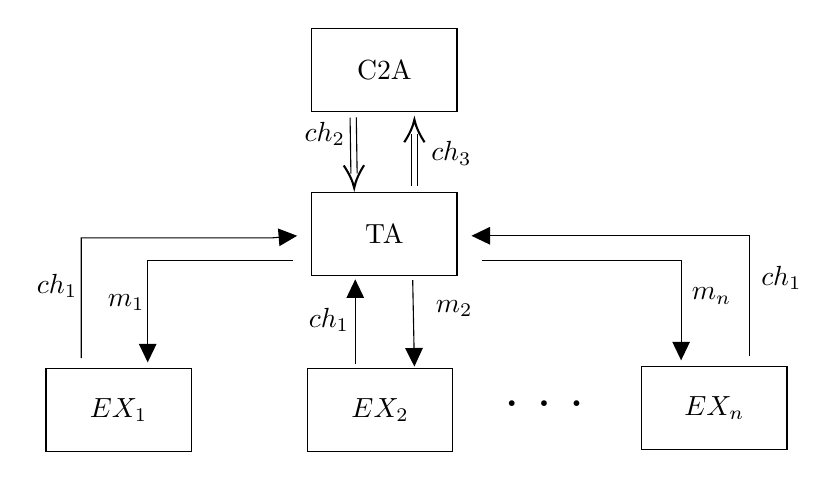
\begin{tikzpicture}[x=0.75pt,y=0.75pt,yscale=-1,xscale=1]
%uncomment if require: \path (0,225); %set diagram left start at 0, and has height of 225

%Shape: Rectangle [id:dp7793135649662085] 
\draw   (146,89) -- (216,89) -- (216,129) -- (146,129) -- cycle ;
%Shape: Rectangle [id:dp8388066725390221] 
\draw   (146,10) -- (216,10) -- (216,50) -- (146,50) -- cycle ;
%Shape: Rectangle [id:dp48691256180587716] 
\draw   (18,174) -- (88,174) -- (88,214) -- (18,214) -- cycle ;
%Straight Lines [id:da7136052167478543] 
\draw    (194.67,131.33) -- (195.44,170) ;
\draw [shift={(195.5,173)}, rotate = 268.85] [fill={rgb, 255:red, 0; green, 0; blue, 0 }  ][line width=0.08]  [draw opacity=0] (8.93,-4.29) -- (0,0) -- (8.93,4.29) -- cycle    ;
%Straight Lines [id:da1199439366931846] 
\draw    (35,169) -- (35,111) -- (127,111) -- (136.01,110.25) ;
\draw [shift={(139,110)}, rotate = 535.24] [fill={rgb, 255:red, 0; green, 0; blue, 0 }  ][line width=0.08]  [draw opacity=0] (8.93,-4.29) -- (0,0) -- (8.93,4.29) -- cycle    ;
%Shape: Rectangle [id:dp8070909053866772] 
\draw   (305,173) -- (375,173) -- (375,213) -- (305,213) -- cycle ;
%Shape: Rectangle [id:dp18131918632628874] 
\draw   (144,174) -- (214,174) -- (214,214) -- (144,214) -- cycle ;
%Straight Lines [id:da23459308482895536] 
\draw    (357,168) -- (357,110) -- (226,110) ;
\draw [shift={(223,110)}, rotate = 360] [fill={rgb, 255:red, 0; green, 0; blue, 0 }  ][line width=0.08]  [draw opacity=0] (8.93,-4.29) -- (0,0) -- (8.93,4.29) -- cycle    ;
%Straight Lines [id:da9340034396500284] 
\draw    (228,122) -- (324,122) -- (324,167) ;
\draw [shift={(324,170)}, rotate = 270] [fill={rgb, 255:red, 0; green, 0; blue, 0 }  ][line width=0.08]  [draw opacity=0] (8.93,-4.29) -- (0,0) -- (8.93,4.29) -- cycle    ;
%Straight Lines [id:da26523318096149495] 
\draw    (137,122) -- (67,122) -- (67,168) ;
\draw [shift={(67,171)}, rotate = 270] [fill={rgb, 255:red, 0; green, 0; blue, 0 }  ][line width=0.08]  [draw opacity=0] (8.93,-4.29) -- (0,0) -- (8.93,4.29) -- cycle    ;
%Straight Lines [id:da6224238934860249] 
\draw    (167,172) -- (167,134) ;
\draw [shift={(167,131)}, rotate = 450] [fill={rgb, 255:red, 0; green, 0; blue, 0 }  ][line width=0.08]  [draw opacity=0] (8.93,-4.29) -- (0,0) -- (8.93,4.29) -- cycle    ;
%Straight Lines [id:da30878293142018354] 
\draw    (167.5,52.98) -- (167.9,79.98)(164.5,53.02) -- (164.9,80.02) ;
\draw [shift={(166.5,87)}, rotate = 269.15999999999997] [color={rgb, 255:red, 0; green, 0; blue, 0 }  ][line width=0.75]    (10.93,-4.9) .. controls (6.95,-2.3) and (3.31,-0.67) .. (0,0) .. controls (3.31,0.67) and (6.95,2.3) .. (10.93,4.9)   ;
%Straight Lines [id:da1036410124215259] 
\draw    (197,61) -- (197,86)(194,61) -- (194,86) ;
\draw [shift={(195.5,54)}, rotate = 90] [color={rgb, 255:red, 0; green, 0; blue, 0 }  ][line width=0.75]    (10.93,-4.9) .. controls (6.95,-2.3) and (3.31,-0.67) .. (0,0) .. controls (3.31,0.67) and (6.95,2.3) .. (10.93,4.9)   ;

% Text Node
\draw (181,30) node   [align=left] {C2A};
% Text Node
\draw (181,109) node   [align=left] {TA};
% Text Node
\draw (53,194) node    {$EX_{1}$};
% Text Node
\draw (23.33,134.33) node    {$ch_{1}$};
% Text Node
\draw (214.67,145) node    {$m_{2}$};
% Text Node
\draw (340,193) node    {$EX_{n}$};
% Text Node
\draw (179,194) node    {$EX_{2}$};
% Text Node
\draw (258,191) node  [font=\Large] [align=left] {\textbf{. . .}};
% Text Node
\draw (338.67,139) node    {$m_{n}$};
% Text Node
\draw (56.67,142) node    {$m_{1}$};
% Text Node
\draw (154.33,150.33) node    {$ch_{1}$};
% Text Node
\draw (372.33,130.33) node    {$ch_{1}$};
% Text Node
\draw (152.33,60.83) node    {$ch_{2}$};
% Text Node
\draw (213.33,70.33) node    {$ch_{3}$};


\end{tikzpicture}}
    \caption{Channel System Representation}
    \label{fig:CS}
\end{figure}